Linebacker 2

DESIGNER: Claes Henrikson
Graphics: Fredrik P. Malmberg
Copyight ©1979
Swedish Game Production

\section*{INTRODUCTION}
LINEBACKER 2 is a strategic game
of the bombing of North Viet Nam in
late 1972.

\section*{SETTING UP THE GAME}
First, see scenario instructions for
information on the forces available
to each player. The North Vietnamese
(NV) player divides his fighter unit
counters between his air bases on his
air status display. Two units (four
planes) may begin the game in the
air, represented on the game map by
its proper echo marker (see move-
ment). He then proceeds to indicate
the number of available Anti-Aircraft
missiles on his SAM SUPPLY TABLE.
The United States (US) player
divides his available air units between
the target boxes on his air status
display and places the corresponding
echo counters face-down in the US
holding area on the game map.

%  Define a macro for inserting the graphic
\newcommand{\bfiftytwo}{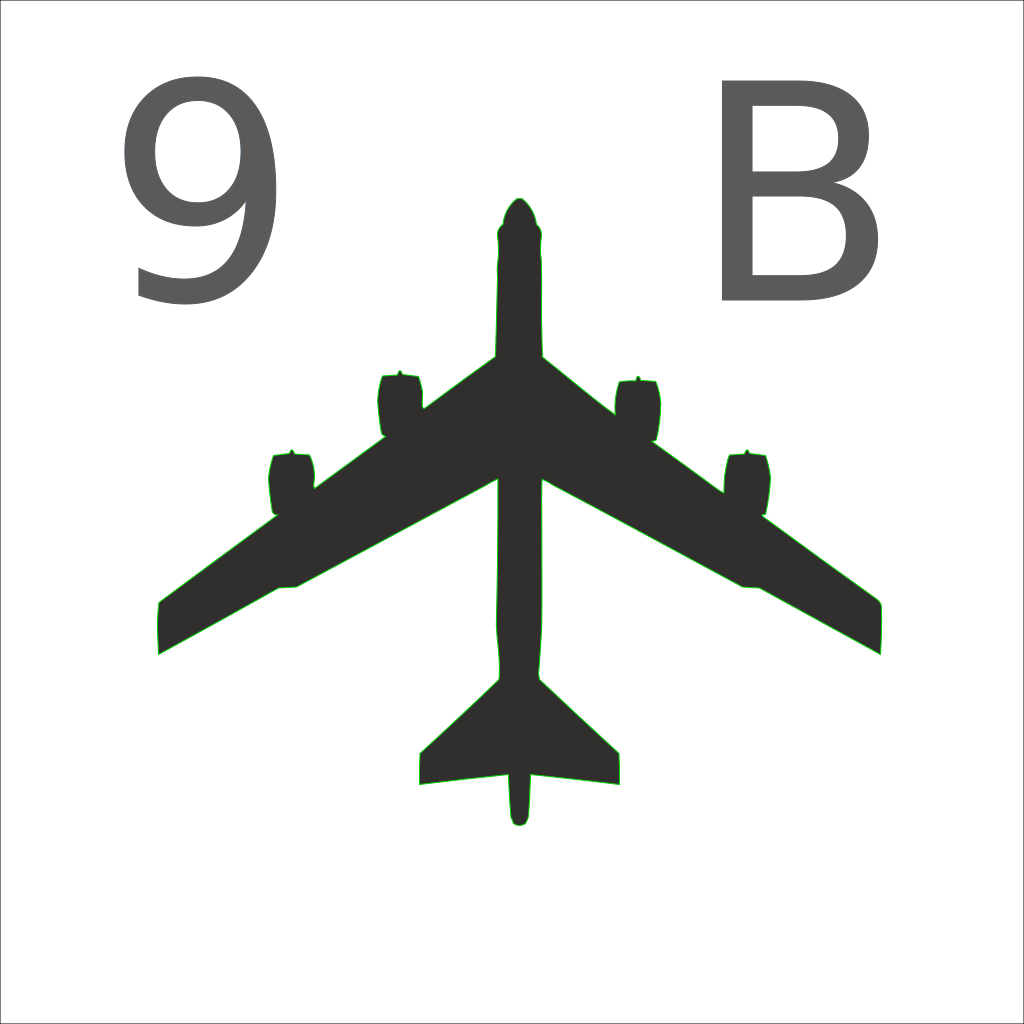
\includegraphics[width=0.25in]{../counters/b52-counter.pdf}}
\newcommand{\ffour}{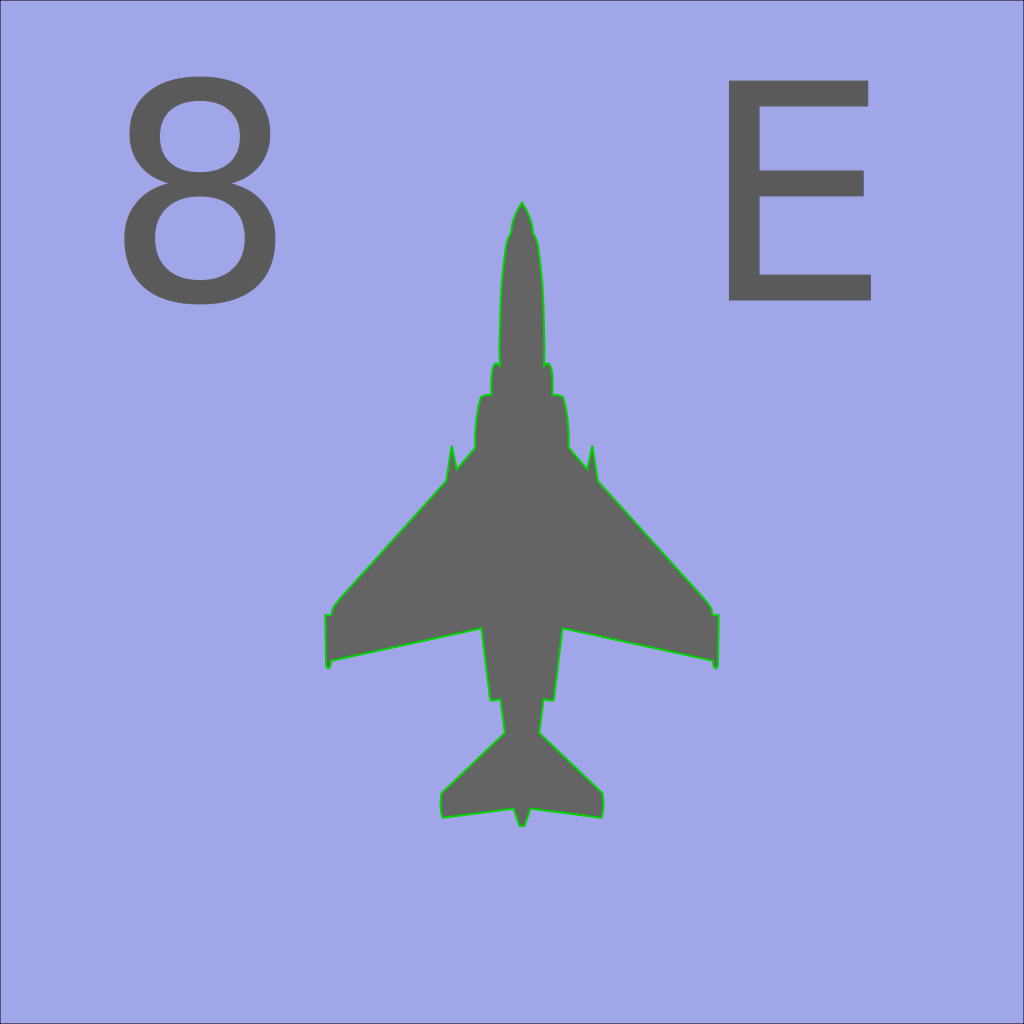
\includegraphics[width=0.25in]{../counters/f4-counter.pdf}}
\newcommand{\foneeleven}{
\includegraphics[width=0.25in]{../counters/f111-counter.pdf}}
\newcommand{\plus}{
\includegraphics[width=0.25in]{../counters/plus-counter.pdf}}
\newcommand{\migtwoone}{
\includegraphics[width=0.25in]{../counters/mig21-counter.pdf}}
\newcommand{\radar}{
\includegraphics[width=0.25in]{../counters/radar-counter.pdf}}
\newcommand{\hit}{
\includegraphics[width=0.25in]{../counters/hit-counter.pdf}}
\newcommand{\graphic}{
\includegraphics[width=0.25in]{../counters/plus-counter.pdf}}

\section*{UNITS}
\noindent
\begin{tabularx}{\linewidth}{@{} m{0.3in} X @{}}
   \radar & Radar Echo \# - confirms to MISSION DISPLAY \#indicator \\
   \bfiftytwo & 3 B-52 bombers \\
   \foneeleven & 4 F-111 strike aircraft \\
   \ffour & 8 F-4 strike fighters/escort fighters \\
   \plus & 1 A-6 EMC aircraft \\
\end{tabularx}

\noindent
\begin{tabularx}{\linewidth}{@{} m{0.3in} X @{}}
   \hit & 1 aircraft downed \\
   \migtwoone & 2 MiG-21 fighters \\
   \graphic & SAM supply indicator [hundreds, tens, and ones] \\
 \end{tabularx}

% \section*{SEQUENCE OF PLAY}
% 1. First SAM fire phase
% 2. Air-to-Air combat phase:
%    A. Interception segment
%    B. B-52 defensive fire segment
%    C. Air superiority segment
% 3. Bombing phase:
%    A. Low-level flak attack segment
%    B. Bombing phase
% 4. Movement phase:
%    A. First player movement segment
%    B. Second player movement segment
% 5. Second SAM fire phase
% 6. Record the passage of one GAME TURN


\section*{SEQUENCE OF PLAY}
\begin{enumerate}[nosep]
    \item First SAM fire phase
    \item Air-to-Air combat phase:
        \begin{enumerate}[nosep]
            \item Interception segment
            \item B-52 defensive fire segment
            \item Air superiority segment
        \end{enumerate}
    \item Bombing phase:
        \begin{enumerate}[nosep]
            \item Low-level flak attack segment
            \item Bombing phase
        \end{enumerate}
    \item Movement phase:
        \begin{enumerate}[nosep]
            \item First player movement segment
            \item Second player movement segment
        \end{enumerate}
    \item Second SAM fire phase
    \item Record the passage of one GAME TURN
\end{enumerate}


Each game turn is divided into
several phases. Follow the above
sequence every game turn performing
actions as per the rules given for each
phase.

\section*{SAM FIRE}
All SAM fire takes place during the
two SAM FIRE PHASES. The NV
player may fire SAMs at all, any or
none of the US echo counters in a map
box (except the US HOLDING AREA
Box). He decides the number of SAMs
fired in each salvo and resolves
combat on the proper column of the
FLAK CRT, subtracting the number
of fired SAMs on the SAM SUPPLY
TABLE.

An echo counter may only be fired
at once in every SAM Fire Phase.
\section*{FLAK CRT}

The dice roll column on the extreme
left of the Flak CRT represents six of
the twenty-one possible outcomes of
two simultaneously rolled six-sided
dice. (The other fifteen outcomes are
considered ``no effect'' and are
deleted for practical purposes.)

The numbers on the top line
represent the number of SAMs fired
in a salvo. The numbers at the inter-
sections between the lines and
columns are the numbers of aircraft
hit and downed by the salvo. If tar-
get is B-52 or ECM aircraft only the
four ``boxed-in'' results on the CRT
are valid.

The Low-Level Flak CRT is only
used against F-111 or F-4 echo
counters attacking targets. The NV
player rolls two dice and consults the
Low-Level Flak CRT for the result. If
an ECM aircraft is present in the
attacking echo counter. he uses the
``ECM'' column, in other cases the
``Normal'' column.

\section*{AIR-TO-AIR COMBAT}

Friendly air units (NV fighters or US
Air Superiority Missions only) may
attack enemy air units in the same
map box, during the Air-to-Air
combat phase. This phase starts with
the NV. player announcing what
echos he is going to attack. The US
player then flips the attacked echo
counters to reveal their echo number
and what aircraft they contain. The
NV player then rolls two dice and
consults the Air-to-Air CRT for re-
sults. The US player places the re-
sulting number of HIT markers in the
corresponding box on his Air Status
Display. If the echo counter contains
B-52’s the US player rolls two dice
for each B-52 in the box before the
attack and consults the ``B-52 Defen-
sive Fire'' column on the Air-to-Air
CRT, and the NV player places the
resulting number of HIT markers in
the corresponding boxes on his Air
Status Display. This is repeated
until all NV attacks are resolved.
The US player then announces his
attacks on NV air units, rolling two
dice and consulting the proper line
on the Air-to-Air CRT for results.
Note that the results “2” through
“6” are deleted from the CRT. They
are considered “no effect.”
F-111 and F-4 units on bombing or
strafing missions attacked by NV
fighters are considered to drop their
ordnance and join the fight. After
the fight they must head for the US
holding area.
Air superiority missions may never
bomb, and must return to Holding
Area after a fight.
NV fighters must return to “home
base” after attack.

\section*{BOMBING}
All bombing takes place in the bomb-
ing phase. US fighters dropping
ordnance to join in air-to-air combat is
not considered as bombing.
At the beginning of the Bombing
Phase, the US player states which
units will bomb and their targets,
flipping the echo counters to reveal
their numbers. All F-4 and F-111
missions are considered to be low-
level attacks and must go through the
Low-Level Flak Attack segment before
they can bomb. The result of the NV
Flak Fire is applied immediately
(before resolution of bomb-run) and
hit markers placed in the proper
display boxes.
The US player then resolves each
echo counter’s bomb run on the
BOMBING TABLE using the proper
target and bombing strength columns,
rolling two dice and adjusting the
dice roll for Pilot Morale. Note that
bombing of Hanoi-Haiphong or other
towns may lead to NEGATIVE
victory point totals.
Numbers in AIRFIELD bombing
table represent aircraft destroyed on
the ground, and only apply to air-
craft in Airfield Alert or Landing/Turn
around boxes on NV player air status
display of airfield attacked. “S”
means airfield destroyed and may not
be used for remainder of game.
No “target of opportunity” bomb-
ing is allowed; a unit must bomb the
target it is targeted for on the US air
status display.

\section*{MOVEMENT}
Movement may only take place dur-
ing the movement phase. All units
have a uniform movement allowance
of “one”, enabling them to move
from one map box to another, crossing
the dividing lines or moving along the
lines connecting the map boxes and
the US HOLDING AREA BOX. No
diagonal movement is allowed.
NV air units begin the game in the
airfield alert boxes of the NV air
status display (exception: see setting
up the game). In his movement
phase, the NV player may move all,
any, or none of his aircraft counters
into the “take-off” box, placing the
appropriate echo counters on the
game map, in the map box contain-
ing the airfield of the unit. The echo
counter may then move in the coming
game turns according to the move-
ment rules. The fighter unit/stack of
units must move one step on the
display boxes for each game turn
(movement phase) in the air, and in
the Movement Phase it enters the
Landing/Turn-around box, must
return to its home airfield. If the air
unit cannot return, i.e., the echo
counter is in another map box than
the home airfield, the unit(s) is
removed from play and may not
return till the next day (night, really)
first GT. If the unit ends up in the
South China Sea map box with air-
craft counter in “landing” box, the
aircraft are permanently lost, ceding
victory points to US player.
No airfield may have more than one
echo counter on the game map at
the same time.

No NV units may enter the US
Holding Area Box.

US echo counter have unlimited
staying power (=9 GTs) on the map,
but must return to US holding area
after they have bombed or entered
air-to-air combat (except 8-52 which
only returns after they have bombed).

Units left on the map after the end
of the ninth GT are removed and
placed in the air status display for
the next night (exception: NV units in
South China Sea box as above).

\section*{US PILOT MORALE}
Pilot Morale (PM) is measured on a
6-0 scale where ‘’6’’ is good and
“0’’ is lousy. PM drops one level tor
every flight of B-52’s taking losses
(for this purpose, one echo counter
equals one flight), and raises one
level for every 250 SAMs fired or
seven continuous nights without B-52
missions. PM only affects B-52
missions results.
PM effects:
6o0r.5 No effect
4 or 3 Subtract ‘/1’’ from bombing
dice rolls
2 or 1 Subtract ‘’2’’ from bombing
dice rolls
0 No B-52 missions allowed

\section*{THE GAME-TURN TRACK}
LINEBACKER II is played in game
turns, each GT consisting of the six
phases making up the Sequence of
Play. Nine GTs make up one night of
real time. No DAYLIGHT GTs are
played. After the ninth GT is com-
pleted, the playing pieces are re-
moved from the game map and set up
on the air status display anew (see
Movement Rules).
\section*{VICTORY POINTS}
Each downed aircraft gives victory
points as follows:
B-52: 10 VP
F-111 or ECM: 2 VP
F-4 or NV fighter: 1 VP
Other VPs as of Bombing Tables,
and:
Destroyed airfield: 5 VP
US PM hits ‘0’: 20 VP to NV player
First bombing of Hanoi/Haiphong:
10/5 VP to NV player

\section*{SCENARIOS}
1. Campaign scenario
Date: 17/12 - 28/12
US Forces:
132 B-52
30 F-111
182 F-4
NV Forces:
40 fighters
1000 SAMs
Airfields intact
US player is first player, US PM: 6
Reinforcements: US, 24/12 7 ECM
aircraft
Victory conditions:
[Victory Point Totals]
US:
0-10 Draw
11-20 Business as usual
21-30 Tactical victory—Fly the
friendly skies of Nam
31+ War won militarily to be lost
by politicians
NV:
0-10 Draw (victory, really!)
20-11 Tactical victory
21-30 Strategic victory: Go south and
win the war

2. First Phase Scenario
Date: 17/12 - 24/12
Forces: as campaign
Victory conditions: as campaign
Special rule: 20 VP to US player if
SAM supply falls below 300
3. Second Phase Scenario
Date: 25/12 - 28/12
US Forces:
123 B-52
28 F-111
120 F-4
6 ECM aircraft
NV Forces:
32 fighters
400 SAMs
Airfields 2 and 6 destroyed
Victory points: 30 to VN player,
US PM: 4
Victory conditions: as campaign game

TAU CETI 2015AD
“We designed TAU CETI because we were fed up
with all the hypercomplex Science Fiction games
out today. With the present ‘state of the art’
surely it must be possible to design a game
simple in play yet with a complex game system?
We think we have succeeded.”
Tau Ceti is a challenging SF game simulating tactical ground
combat on an alien planet in the year 2015. The two different
races, Kra (red lizard-type and vicious, but with two legs) and
H’ren (blue-furred mouse-like creatures but with two arms
and two legs) fight for control of the planet and employ two
different tactics: Kra employing strong Plasma Launchers
and Heavy Assault Vehicles—and H’ren using hordes of Light
Assault Vehicles and Hovercarriers.
Three terrain levels and three altitude levels enable the play-
ers to fight a semi-three dimensional battle and without paper-
work—a simple marker tells you on which altitude a unit is on.
Hovering, transportation, two different combat doctrines (P
and I Combat), line of sight, spotting, remotes (ground/aerial
bombs/mines) all play important roles to make this game a fun
and fast-playing “simulation”. And don’t forget the ten
scenarios. These will keep you playing till the first astronaut
steps on Mars!
A high level of physical quality is maintained. The three-color
map is printed in tints of black, green, and brown. The 130
back-printed die-cut counters are three-colored and bear
silhouettes of the combat units. The rulebook is illustrated and
typeset. Last but not least, the front cover bears a wonderful
illustration by the artists. Eddie Eddings and Jim Newsome
(and a drawing of Jim’s appears inside the game). Our game
is packaged in a ziplock bag for easy storage and to keep the
price low. In fact, ridiculously low.
The game is available through larger stores around the world,
or directly from us:

SWEDISH GAME PRODUCTION
Box 18
S-590 40 Kisa, Sweden

